%!TEX root = thesis.tex

\chapter{Exploratory Field Study}
\label{chap:exploratory-field-study}

\begin{figure}
\centering
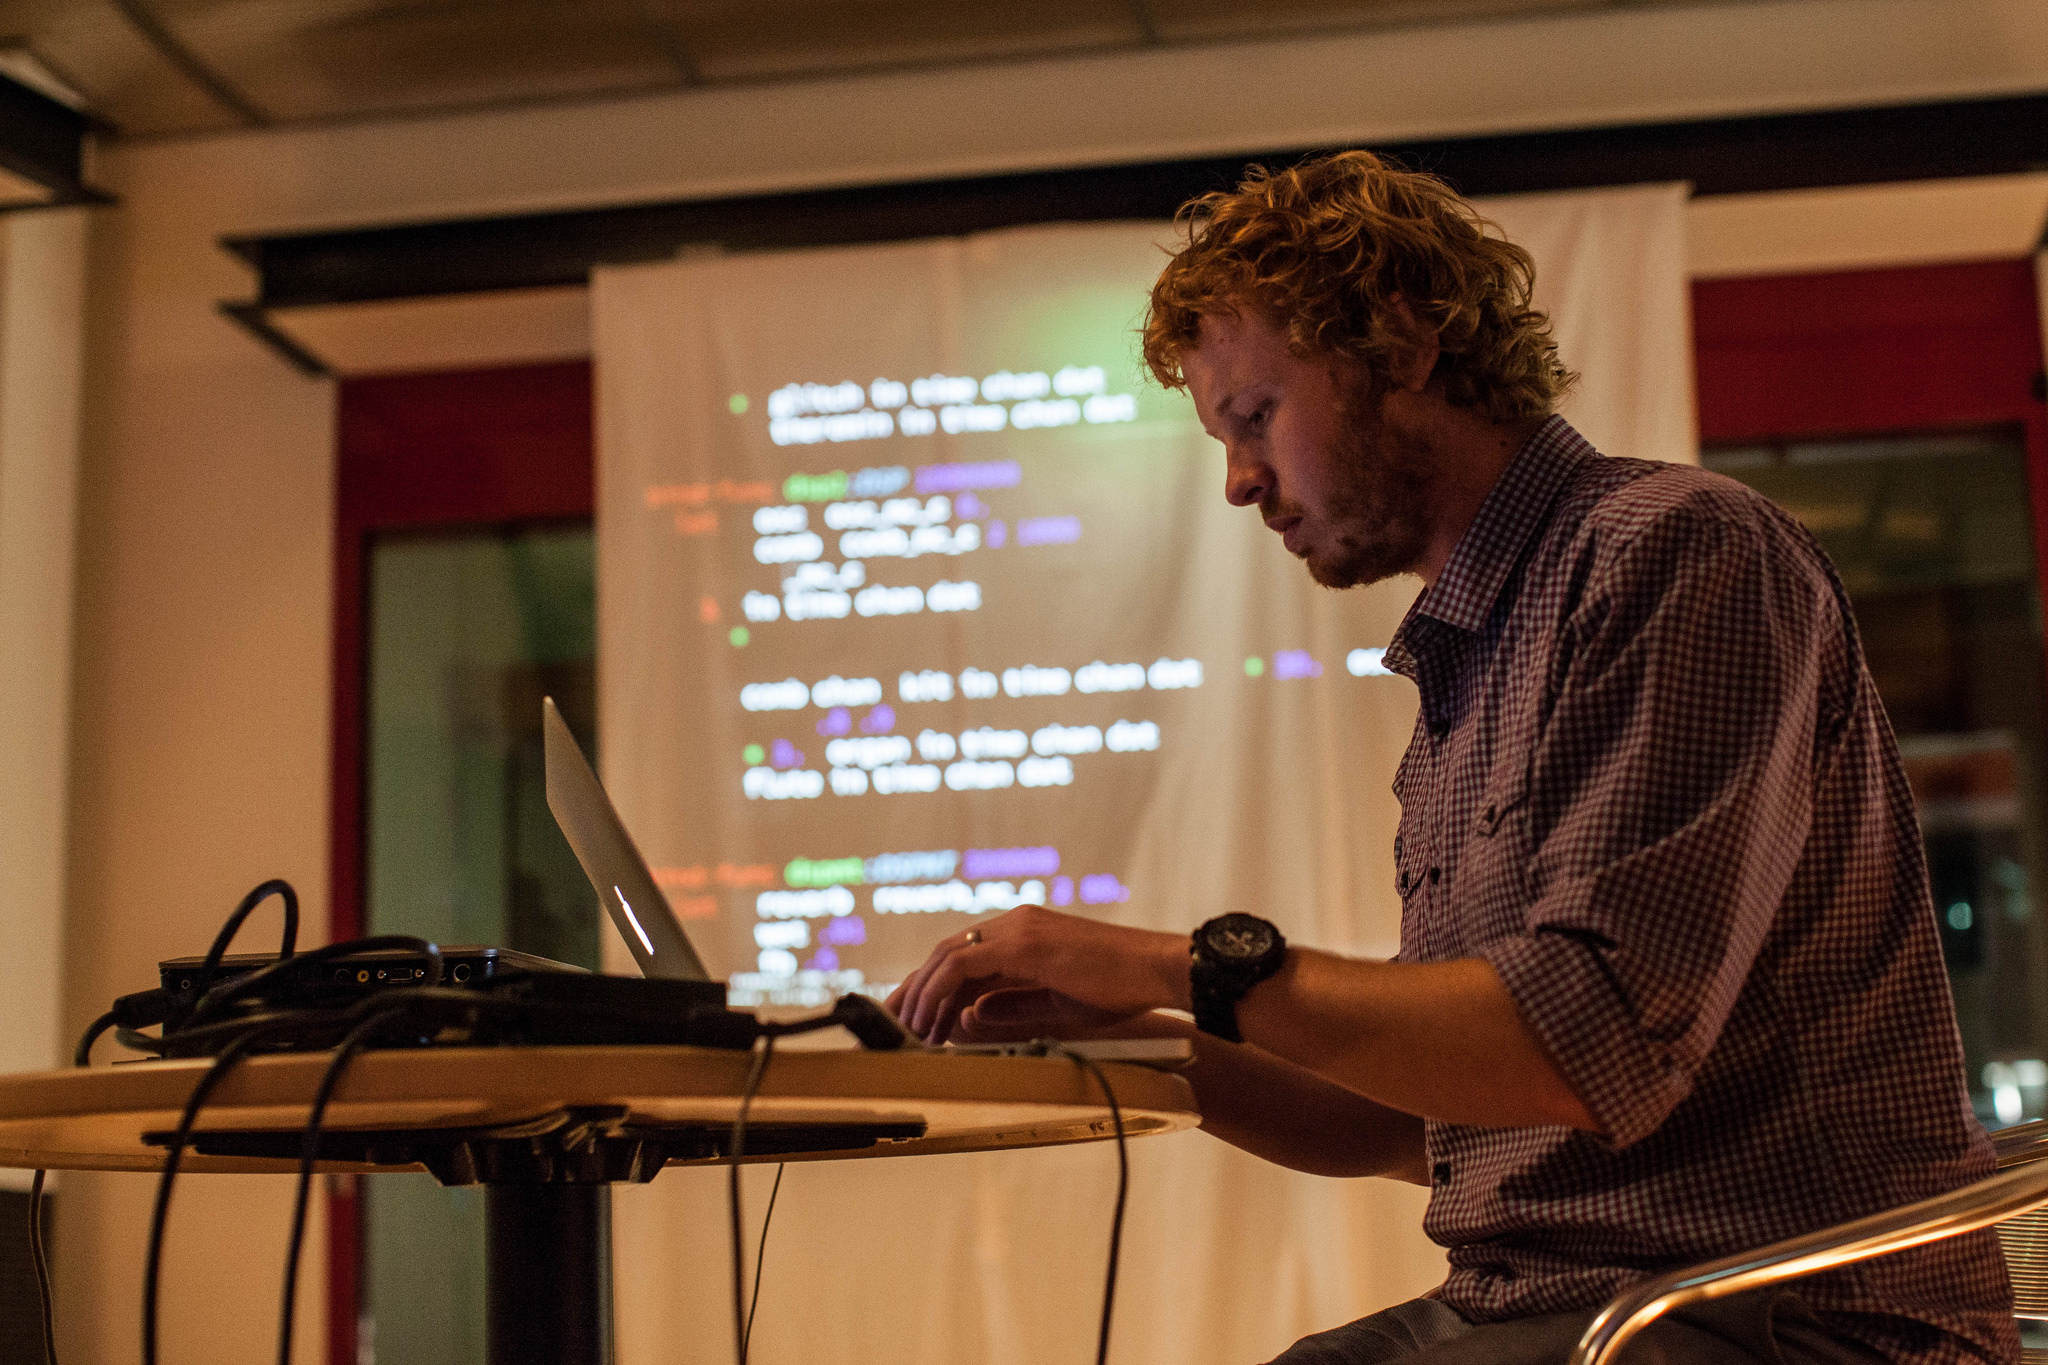
\includegraphics[width=1.0\textwidth]{../images/study-1-you-are-here-ben.jpg}
\caption[Standard live coding setup]{The standard live coding setup includes a laptop connected to a projector (pictured in foreground) displaying program source code (pictured in background) to an audience.}
\label{fig:exploratory-field-study-ben}
\end{figure}


In order to determine a strategy for visualising source code an exploratory field study was conducted at the ``You Are Here'' arts festival in Canberra (see Figure~\ref{fig:exploratory-field-study-ben}). The literature identified the need to re-examine existing models of visualisation and develop a strategy for implementing visualisations within the space of live coding. To this end, an exploratory field study examined the existing understanding and enjoyment (as discussed in~\cite{McLean2010a}) of a live coding audience via a survey distributed after a performance. This examined the live coding performance with only the source code projected without any visualisation. This would provide a baseline for the addition of visualisations to live coding.

In addition to the survey distributed during the performance a set of follow-up email-based interviews were conducted. The purpose of these interviews was to gain insight into the audience's current understanding and enjoyment of the live coding process. Additionally, the relationship between enjoyment and understanding was to be examined. It was hoped that the examination of these factors would further inform the development of visualisations targeted at similar audiences and lead to a more general software visualisation strategy.

\section{Method}

Audience members were asked to fill out a survey (see Appendix~\ref{appendix:field-study-survey}) regarding their perception of and response to the projection of the computer code during the performance. Each audience member was asked to indicate which of a number of curves or trajectories best represented their \emph{enjoyment} and \emph{understanding} of the performer's actions through the performance. These trajectories allowed for ``high'', ``medium'', and ``low'' levels of enjoyment and understanding for the self-determined ``beginning'', ``middle'' and ``end'' of the performance (see Figure~\ref{fig:field-study-curves}). Additional questions addressed the audience's sense of ``liveness'' of the performance (c.f.~\cite{Auslander}) and whether the projected code was confusing.

Follow-up email questions were distributed following the performance to a number of those in attendance. The follow-up email asked two questions: ``What did you \emph{understand} about what was going on with the code being projected? In particular, what did you understand about the relationship between the code and the music?'' and ``What would you like to understand more about the code in order to enjoy the performance more?''.

% \begin{itemize}
% \item What did you \emph{understand} about what was going on with the code being projected? In particular, what did you understand about the relationship between the code and the music? \qlab{question:study-1-email-understand-relationship}
% \item What would you like to understand more about the code in order to enjoy the performance more? \qlab{question:study-1-email-understand-enjoy}
% \end{itemize}

\begin{figure}
\centering
\fbox{
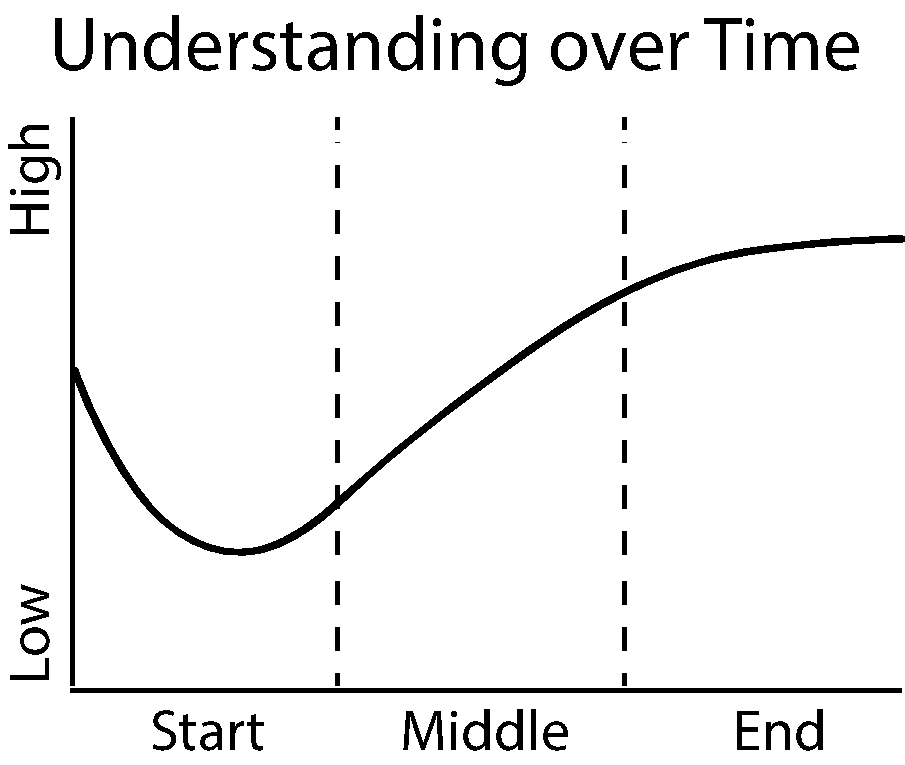
\includegraphics[width=0.3\textwidth]{../study-1/survey/understanding-over-time.pdf}}
\hfill
\fbox{
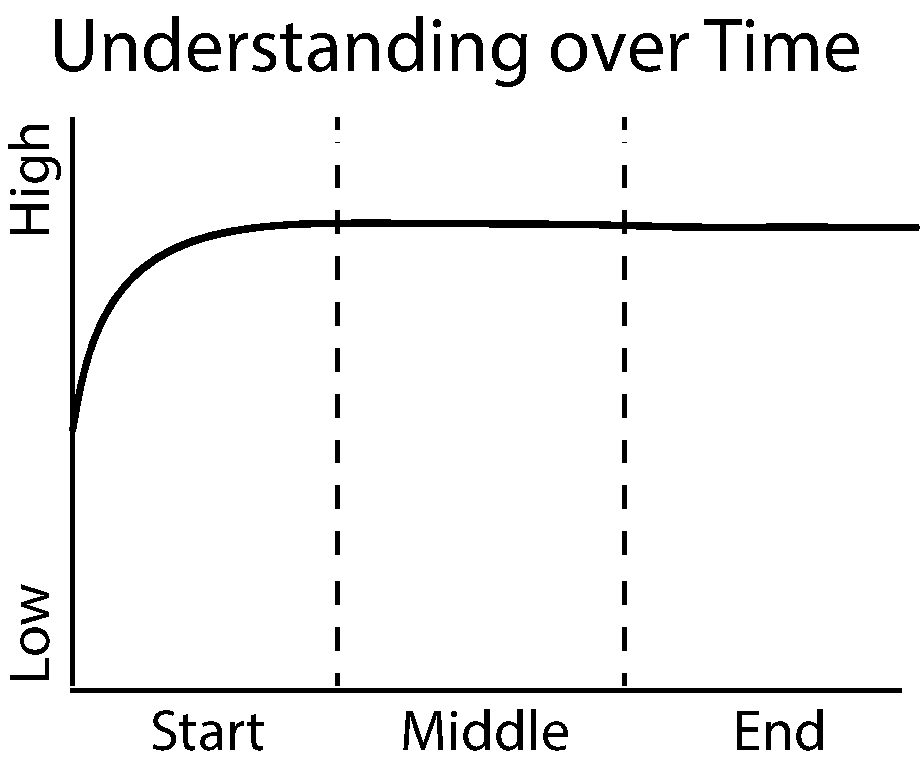
\includegraphics[width=0.3\textwidth]{../study-1/survey/understanding-over-time-2.pdf}}
\hfill
\fbox{
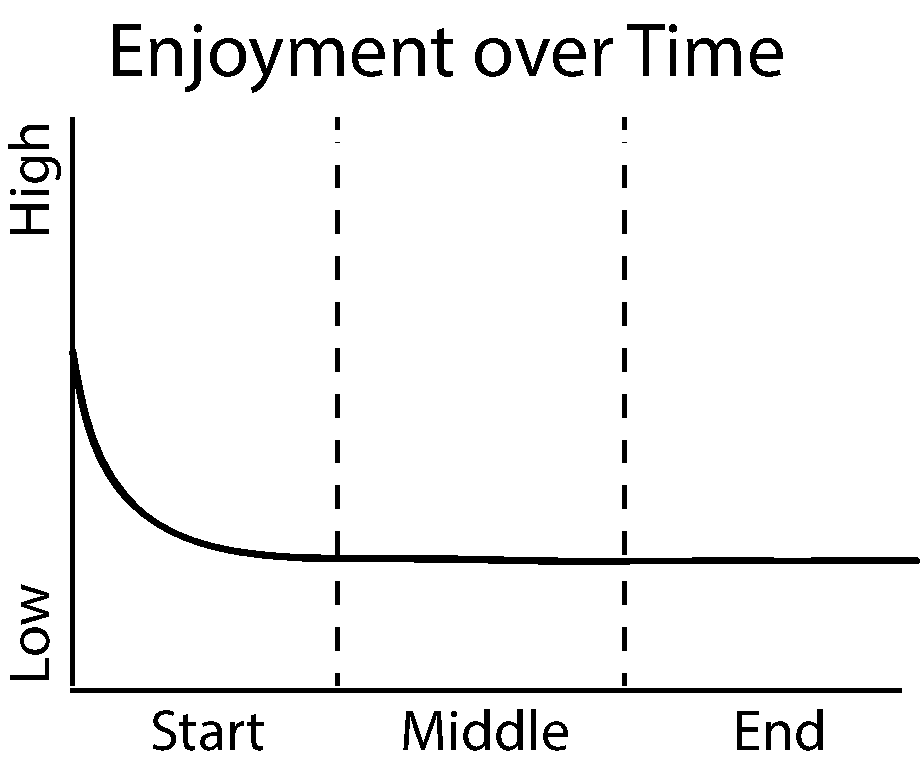
\includegraphics[width=0.3\textwidth]{../study-1/survey/enjoyment-over-time.pdf}}
\caption[Three examples of curves provided to the audience during the
exploratory field study]{Three examples of curves provided to the audience during the
exploratory field study. A total of five curve options were provided for
both dimensions of understanding and enjoyment. For the understanding
dimension, the survey question asked the participants to: ``circle the
image that best represents your understanding of the relationship
between the visuals and the music through the performance.'' For the
enjoyment dimension, the survey question asked the participants to:
``circle the image that best represents your enjoyment through the
performance.''}
\label{fig:field-study-curves}
\end{figure}


\section{Participants}

A total of thirteen survey responses were received. Of these, $77\%$ regularly listen to music and $54\%$ perform regularly. $38\%$ of the respondents stated that they had high exposure to programming through work, study or their hobbies, $31\%$ stated that they had some experience and $31\%$ stated that they had no experience with it. Of the respondents, $69\%$ had never been to a live coding performance before.

$77\%$ stated that they listen to large amounts of music compared to $23\%$ that stated they only listened to a small amount. $54\%$ stated that they performed music reguarly, $16\%$ stated that they performed only occasionally and $31\%$ stated that they had never performed music.

\section{Results}

\subsection{Survey}

Of the thirteen survey responses received, six audience members showed a high level of enjoyment throughout the whole performance, while the remaining seven responses showed alternating levels of enjoyment. No audience members indicated a low level of enjoyment throughout the performance.  Only two of the thirteen respondents indicated that they understood the relationship between the code projections and the music throughout the performance. Three of the six respondents who reported a high level of enjoyment throughout the performance also indicated an increase in understanding (from low to high) as the performance progressed, although a Chi-square analysis revealed no significant relationship between enjoyment and understanding. 

When asked if the projected code helped to communicate a sense of liveness, nine members of the audience indicated that the projected code helped whereas four members of the audience indicated that the projected code had no effect on their sense of liveness.

Regarding confusion, five members of the audience stated that they found no aspects of the visuals confusing. For the members of the audience that found aspects of the performance confusing, aspects identified as confusing included the small font, the difficulty linking changes in the source code to changes in the sound and the flicking between screens. Four members of the audience did not respond to the question.

\subsection{Follow-up Interview}
\label{section:study-1-follow-up-interview}

The follow-up interview identified some gaps in understanding from the survey. A total of three email responses were received. When asked what these audience members felt they understood about the performance, all three responses indicated high understanding of the initial process of building the music from scratch and developing the musical forms to be modified throughout the performance. One of the responses indicated that they could see changes being made but could not identify which elements within the source code related to which elements in the music. Notably, one audience member stated that they didn't ``have a big picture of what all the code looks like'' and this caused them difficulty in understanding the live coding process. 

The second follow-up interview question asked what should be made clearer within the space of live coding prompting a variety of responses. Two audience members stated that more understanding of the ideas or source code changes would be desirable. However, one of the responses indicated that a higher understanding of the live coding performance may result in lower enjoyment and suggested that a higher understanding may take focus away from the enjoyable parts of the performance. 

 % but noted that it may be due to their background and those with less experience in music or programming may find a higher understanding more beneficial.

Results of the follow-up email interview are available in Appendix~\ref{appendix:field-study-follow-up-interviews}.

\begin{figure}
\centering
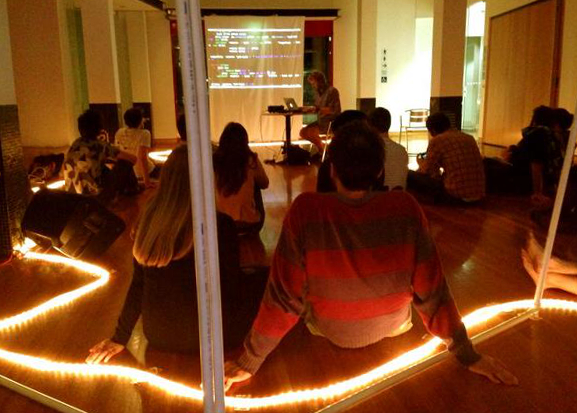
\includegraphics[width=\textwidth]{../images/study-1-you-are-here.jpg}
\caption[A live coder performs at the \textit{You Are Here} arts festival]{A live coder performs at the \textit{You Are Here} arts festival in Canberra.}
\label{fig:you-are-here-performance}
\end{figure}

\section{Discussion}

A large proportion of the audience indicated that the code was confusing. This confusion was confirmed within the follow-up interviews. Despite this confusion, the projected code still conveyed that the programmer was modifying the music indicated by the positive contribution to liveness by the source code identified by $70\%$ of the audience. This was also confirmed within the follow-up interviews in which the interviewees indicated that during the early stages of the performance, the relationship between writing the code and triggering the music was clear.

A number of audience members ($40\%$) stated that they found elements of the source code projections confusing and only a very small number of respondents claimed to have actually understood what the programmer was doing. A small cohort of respondents whose understanding increased through the performance and whose enjoyment remained high suggested that it might be possible to bring more audience members into this group.

\subsection{Limitations}

Due to the layout of the venue, in some locations the projection screen may have been difficult to see. Additionally, the projection screen surface was uneven and due to the projector contrast the projected source code, particularly the punctuation, was difficult to see. This may have contributed to confusion among those with some background in programming.

Results of this study were constrained by sample size. Although the follow-up interview identified some interesting problems within the current live coding practice, it was determined that more could be gained from surveying a larger audience.

In addition, the survey was found to be too limited to make more than basic judgements regarding the audience reported understanding and enjoyment. The survey question asking for the selection of a curve from five options that most closely matched enjoyment and understanding, although providing insight into the audience's opinion of the performance, did not allow for more specific analysis of the stages of the live coding performance.

% These limitations were addressed in following studies.

\section{Summary}

This study identified the need to reduce confusion within the space of live coding. Understanding during the early stages of the performance was shown to be high but drifted as more code was added. During the middle and end of the performance, changes were apparent to the audience but their intention was not clear. The interviewees indicated that an increase in understanding might contribute positively to their experience.

Similarly, this study identified the need to maintain, and if possible increase, levels of enjoyment while attempting to increase understanding. Reported enjoyment was in general high, however, the follow-up interviews identified that some audience members may equally weight the benefits of enjoyment and understanding, suggesting that a focus only on increasing understanding may be detrimental to the live coding performance.

Taken as a whole, this study indicated the need to investigate methods of increasing understanding without reducing enjoyment. The three respondents whose understanding increased through the performance and whose enjoyment remained high indicated that it might be possible to have similar patterns across the wider audience. It was identified that live coding visualisation techniques might contribute to this goal.

% link to stated goal of ``why show the source code at all during a live coding performance?'' and ``are there better methods of demonstrating the programming process?''

